Pixel detectors are semiconductor detectors which are segmented in two dimensions: this distinguishes them from the strip detectors, such that a single plane of detector already provides both the coordinates of impact of the detected particle. 
Their operation is based on the p-n junction (fig. \ref{fig:junction}). 
In an n-doped crystal some silicon atoms are replaced with valence 5 donor atoms (such as P) which provide loosely bound e$^-$ carriers, while in p-doped crystals some atoms are replaced by valence 3 acceptor (such as B) which absorb exixsting free electrons, effectively creating a positively charged carrier called "hole".

A p-n junction is built by bringing in contact two n and p doped silicon crystals. At the boundary, recombination of opposite charge carriers occurs, forming a region, the depletion zone, which is free of charge carriers. The charged donors$^{+}$ and acceptor$^{-}$ atoms, that remain ionised in the n-type and p-type regions, constitute a space charge and create an electric field across the junction, causing a drift current in the opposite direction to the diffusion one, through which the junction reaches an equilibrium state. Assuming a constant space change, the electric field is linear and reach a maximum at the boundary of the $p$ and $n$ layers.
\begin{figure}[h!]
   \centering
   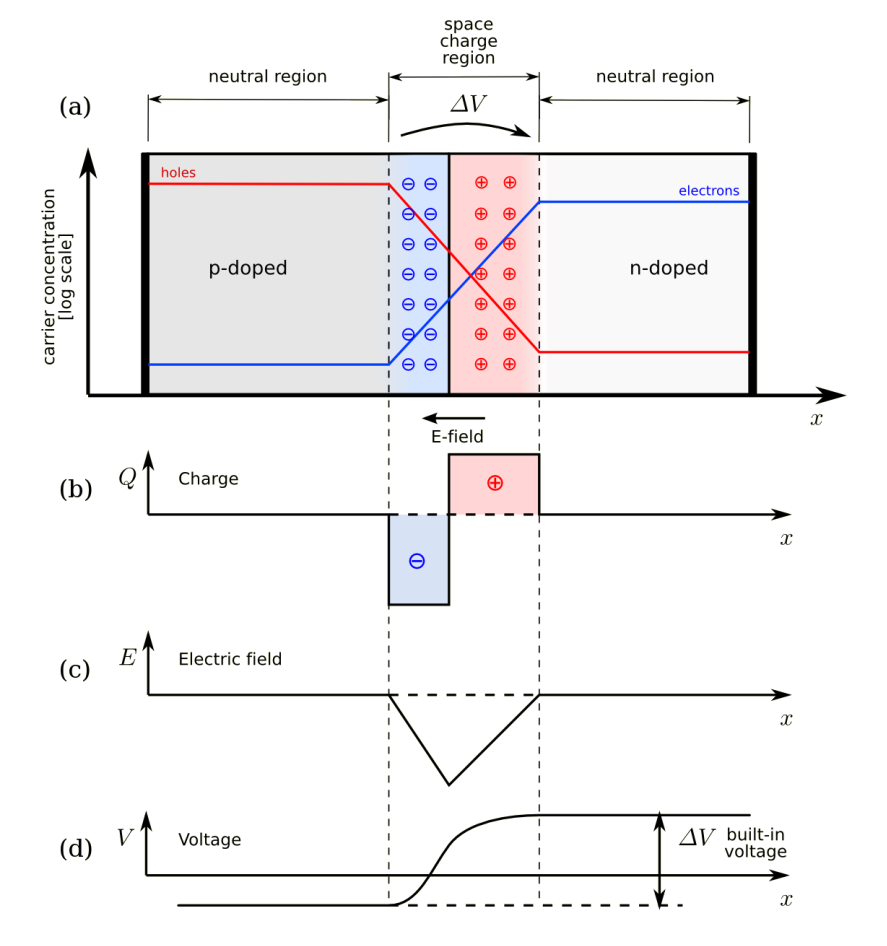
\includegraphics[width=.69\linewidth]{figures/Pixel_detectors/junction.png}
   \caption{The structure of a p-n junction. (a) structure, (b) space charge density, (c) electric field distribution and (d) potential distribution. }
   \label{fig:junction}
\end{figure}
%\red{creation of electron-hole couples in the bulk by the particle impinging which are then separated and drifted by the electric field and collected at their respectively electrodes.
%The applied electric field, the depletion zone thickness, the front end, the processing and the transmittion of the signal are specific charateristics of each particular chip. In this chapter I am going to discuss the main kinds of pixel detectors, dwelling specifically on Monolithic Active Pixels (MAPS).}

\section{Signal formation}
   When a charged particle passes through a semiconductor and loses energy by ionization, only a part of that energy is used to generate electron-hole pairs, since another part is used for other processes, as lattice excitation.
   The average energy needed to create a pair at \SI{300}{K} in silicon is $w_i$ = \SI{3.65}{eV}, that is more than the mean ionization energy because of the interactions with phonons. For a minimum ionizing particle (MIP) the most probable value (MPV) of charge released in the semiconductor is \SI{0.28}{keV/\um}, hence the number of electrons-hole pairs is: 
   \begin{equation}
       \langle \frac{dE}{dx}\rangle \frac{1}{w_i} \sim 80 \: \frac{e/h}{\si{\um}} \sim \frac{1.28 \:10^{-2}\si{fC}}{\si{\um}}
   \end{equation}
   Because of the splitting of the energy depositon between the two different processes, the number $N_{e/h}$ of couples generated undergoes fluctuations that usually follow a Poisson distribution;
   thus the fluctuations of $N_{e/h}$ is equal to  $\sigma_{e/h} =\sqrt{N_{e/h}}$. Since the energy loss is not a purely statistical fact, because of the energy the particle can lose is obviously $\leqslant$E and the energy need for ionization must be $\geqslant$ of the mean ionization energy, the resolution actually is lower by a factor $\sqrt{F}$, where F is called the Fano factor. F is a function of the material and temperature and for silicon is equal to $\sim$0.115.

   In order to avoid a signal loss, pairs e/h must be produced in the depleted region of the semiconductor, where the probability of recombination with charge carriers is low.
   For this reason pixel detectors are commonly reverse biased: a positive bias is given to the $n$ electrode and a negative to the $p$ in order to increase the depletion zone. 
   The width of the depletion region depends on the external bias $V_{ext}$, the resistivity $\rho$ and also with the dopant:
   \begin{equation}
      d_{n} \sim 0.55 \sqrt{\frac{\rho}{\Omega cm}\frac{V_{ext}}{V}} \mu m 
      \hspace{55pt}
      d_{p} \sim 0.32 \sqrt{\frac{\rho}{\Omega cm}\frac{V_{ext}}{V}} \mu m
      \label{eq:deplation_d}
   \end{equation}
   Thus, high resistivity wafers (100 $\Omega cm - k\Omega cm$) are typically preferred because they allow a thicker depletion zone with smaller bias voltage. 

   The charges created whithin the sensor are separated by the electric field and collected at their respective electrodes ($p$ for holes and $n$ for electrons)\footnote{Even if in principle both the electrode can be used to read the signal, for pixel detectors, where the number of channel and the complexity of readout are high, only one is actually used. In strip and pad detectors, instead, is more common a dual-side readout}. A signal $i_e$ is generated on the electrode $e$  by the drift of these charges, as stated by the Shockley-Ramo's theorem: 
   \begin{equation}
        i_e(t) = -q\: v(t)\, E_{WF,e}
   \end{equation}
   where $v(t)$ is the instantaneous velocity of the charge $q$ and $E_{WF}$ is the weighting field, that is the field obtained biasing the electrode $e$ with 1V and all the others with 0V. The drift velocity of the charge depends on the electric field and on the mobility of the particle:
   \begin{equation}
      v = \mu(E)\, E
   \end{equation}
   where $\mu(E)$ is a function of the electric field and is linear in $E$ only for small $E$: at higher values the probability of interactions with optical phonons increases, the mobility drops and this leads to a saturation of the velocity (fig. \ref{fig:mobility_drift}). Typical values for electrons and holes mobility in silicon at room temperature are $\mu _n \sim$\SI{1450}{cm\squared/Vs}, $\mu _h$ = \SI{500}{cm\squared/Vs}.
   \begin{figure}
      \centering
      \begin{subfigure}[b]{0.49\textwidth}
          \centering
          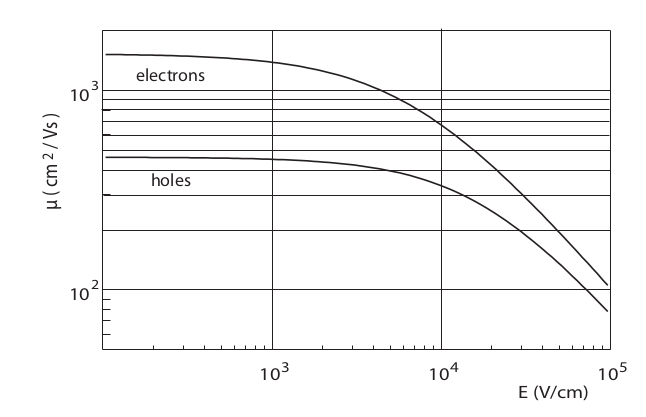
\includegraphics[width=\linewidth]{figures/Pixel_detectors/mobility_in_semiconductor.png}
          \caption{Dependece of the mobility on the electric field.}
          \label{fig:mobility}
      \end{subfigure}
      \hfill
      \begin{subfigure}[b]{0.49\textwidth}
          \centering
          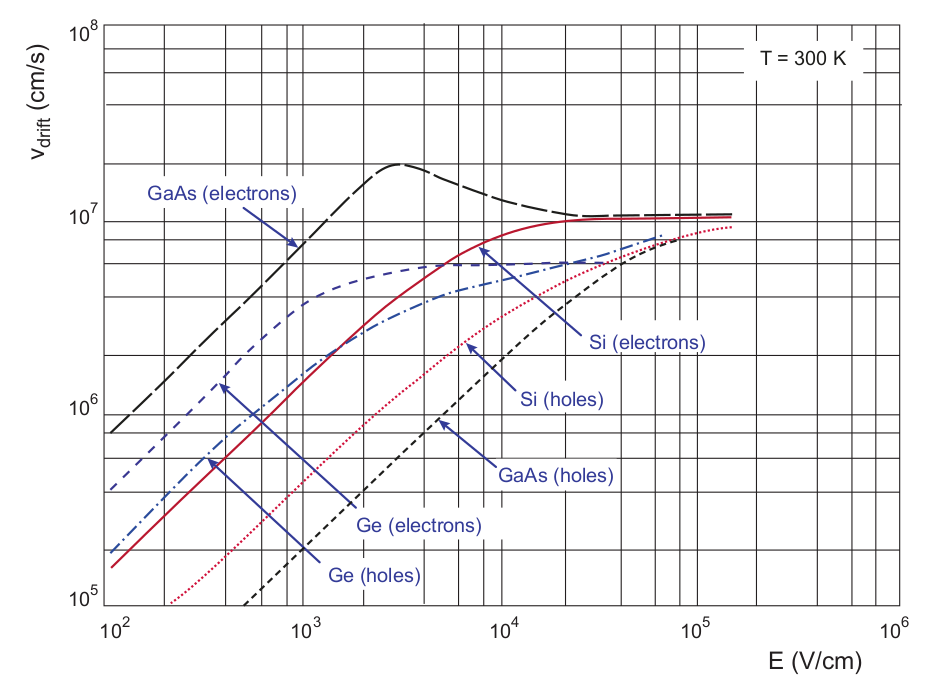
\includegraphics[width=\linewidth]{figures/Pixel_detectors/velocity_in_semiconductor.png}          
          \caption{Drift velocity at room temperature in different semiconductors}
          \label{fig:Drift_velocity}
      \end{subfigure}
         \caption{}
         \label{fig:mobility_drift}
 \end{figure}
 
    
\section{Charge Coupled Devices}
   Charge Coupled Devices (fig.\ref{fig:CCD_scheme}) are one of the first pixel detectors initially developed to detect visible light and then adapted for charged particles and x-rays. 
   In CCDs the charge is created in a very thin active epitaxyal layer (typically \SI{10}{\um}, maximally about \SI{30}{\um}) and then locally stored in a potential minimum which is created by a MOS structure. 
   The size of the CCD cells is typically in the range \SIrange{10}{20}{\um} such that spatial resolutions are of the order of a few micrometres.
   The collected charges are moved stepwise from electrode to electrode (thus so called 'bucket chain') by applying a potential with a clock with frequency of $\sim$\si{MHz}; the readout chain is completely sequential and this makes the entire process comparatively slow (tens of \si{ms}), despite of such high frequency.
   A particular type of CCD, the pnCCDs, are typically used to detect low energy ($<$\SI{10}{keV}) x-ray photons for their homogeneous spatial detection efficiency of photons. The pnCCDs have a sideward depletion similar to silicon drift chambers that makes the electric field stronger, compared with the normal CCDs. 
   The pnCCDs designed for photon imaging are often fabricated with high Z materials, to increase assorbtion efficacy.


   \begin{figure}
      \centering
      \begin{subfigure}[b]{0.49\textwidth}
          \centering
          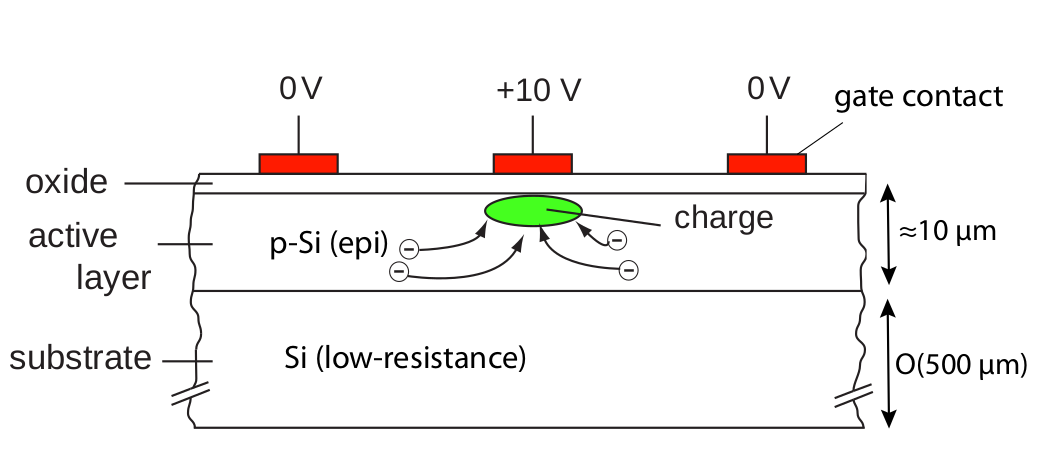
\includegraphics[width=\linewidth]{figures/Pixel_detectors/CCD.png}
          \caption{CCD cross section scheme}
          \label{fig:CCD_scheme}
      \end{subfigure}
      \hfill
      \begin{subfigure}[b]{0.49\textwidth}
          \centering
          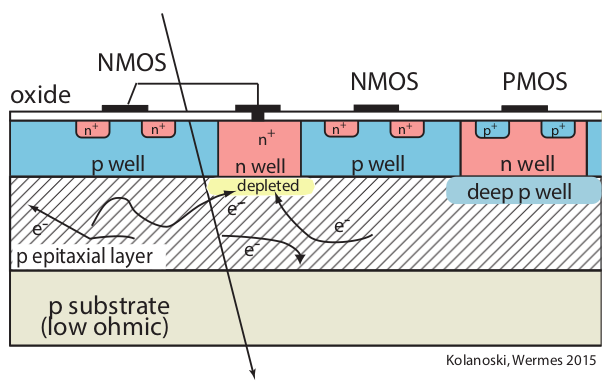
\includegraphics[width=\linewidth]{figures/Pixel_detectors/MAPS_scheme.png}  
          \caption{MAPS cross section scheme}
          \label{fig:MAPS_scheme}
      \end{subfigure}
   \end{figure}


   \begin{figure}
      \centering
      \begin{subfigure}[b]{0.49\textwidth}
          \centering
          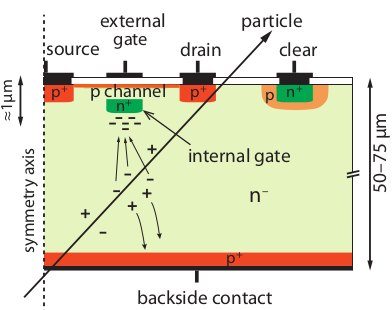
\includegraphics[width=\linewidth]{figures/Pixel_detectors/DEPFET_scheme.png}
          \caption{DEPFET cross section scheme}
          \label{fig:DEPFET_scheme}
      \end{subfigure}
      \hfill
      \begin{subfigure}[b]{0.49\textwidth}
          \centering
          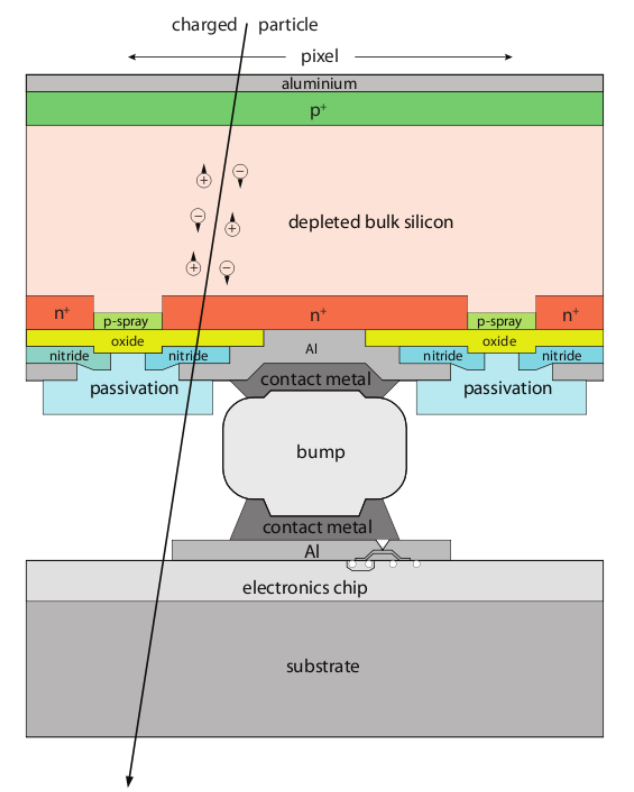
\includegraphics[width=\linewidth]{figures/Pixel_detectors/hybrid_scheme.png} 
          \caption{Hybrid cross section scheme}
          \label{fig:hybrid_scheme}
      \end{subfigure}
   \end{figure}

\section{Hybrid pixels}
   In hybrid pixels, which currently are the state-of-art technology for large scale pixel detectors in most particle physics experiments, the sensors and the electronics are realized on separate wafers and connected together a bump of conductive material, typically In or Sn  (fig. \ref{fig:hybrid_scheme}). 
   They provide a practical system where the sensor and the ASIC (application specific integrated circuit) can be optimized separately, allowing the fabrication of radiation-hard devices capable of operating at \si{GHz} rates.
   However hybrid pixel have also some disadvantages: the bump-bonding interconnet technology is expensive and delicate; the separate substrates for electronics and sensor lead to an increase in the material budget; the pixel dimension must be long enought for the bump-bonding technology, with a current limit of about \SI{50}{\um}.
   %For reasons related with the historical development, the n$^+$-in-n sensors were the first to be used; they demanded double-sided processing which guardanties the detector functionality both before and after the type inversion of the n$^-$ doped bulk into p-type after high quantity of radiation.
   %The pn-diode is initially on the unstructured backside of the sensor, while after, the depletion zone grows from the electrode side into the bulk. This ensures that the signal can be sensed on the pixels even if the substrate is no longer fully depleted, even though the bias voltage required for a sufficient depletion increases, liming the detector lifetime up to a few years.
   %With the availability of high quality p-substrate material ($\gtrsim$\SI{2}{k\Omega cm}) the fabrication of n-in-p type sensors, which does not invert anymore, became the preferred choise leading also a huge advance in cost reduction due to no more need of double sided.
   %However, the particular and sophisticated procedure to bond sensor and ASIC makes them difficult to produce, delicate (especially when exposed to high levels of radiation) and also expensive. 

   DEPFETs are the first attempt towards the integration of the front end (FE) on the same substrate of the sensor.
   Each pixel implements a MOSFET (metal-oxide-semiconductor field-effect transistor) transistor (a p-channel in fig. \ref{fig:DEPFET_scheme}): the hole current flows from source to drain is controlled by the external gate and the internal gate together. The internal gate is made by a deep $n+$ implant towards which electrons drift after being created in the depletion region; the accumulation of electrons in the region underneath the n implant changes the gate potential and controls the transistor current, resuling in an internal amplification, the removal of the signal charge from the internal gate is called "Clear". 
   DEPFET typically have a good S/N ratio: thanks to the on-pixel amplification, to the thick depletion region. 
   As in CCDs, DEPFET require a serial readout of the pixel signal, and are therefore relatively slow devices, but they can be made very think (\SI{50}{\um}).
   In recent years, the sensor development was driven by an intensive R$\&$D and prototyping for x-ray imagers and the ILC vertex detector. 
   

\section{CMOS MAPS and DMAPS}\label{sec:MAPS_DMAPS}
   Monolithic active pixels (fig \ref{fig:MAPS_scheme}) accommodate on the same wafer both the sensor and the FE electronics, with the second one implanted on top within a depth of about \SI{1}{\um} below the surface. 
   MAPS have been first proposed and realized in the 1990s and their practical usage has been enabled by the development of the consumer electronics sector, which guarantees the halving of CMOS transistors dimension at least every two years, as stated by the Moore's law.
   As a matter of fact the dimension of components, their organization on the pixel area and logic density are important issues for the design and for the layout.
   Compared to CCDs, the readout time is dramatically reduced by the in-pixel amplification and discrimination, typically followed by a sparsified readout selecting only over threshold pixels and avoiding the need for signal transporation over thousands of pixels.

   A critical parameter for accelerator experiments is the material budget, which represents the main limit factor for momentum measurement resolution in a magnetic field; since hybrid pixels are thicker ($\sim$ hundreds of \si{\um}) than monolithic ones (even less than \SI{100}{\um}). Using the latter the material budget can be reduced to a third: typical values for hybrid pixels is 1.5 \% $X_0$ per layer, while for monolithic 0.5 \% $X_0$. Compared to MAPS, among other disadvantages of hybrid pixels there is the bigger power consumption, that requires also a bigger cooling system, leading to a futher increase of material.
   %Discorso fatto con Ludovico
   %sul fatto che i CMOSS tirano meno rispetto al circuito analogico.
   %Scrivi perchè si usano i CMOSS invece dei transistor: discorso sulla potenza e sull'elettronica digitale.\\      
   %UNA COSA (TROVATA SULLE SLIDES IFIP DI FORTI)È CHE ELETTRONICA RICHIEDE BASSA RESISTIVITÀ MENTRE ALTA RHO È RICHIESRA PER IL SENSORE. UN ALTRO PROBLEMA DEL CONNUBIO TRA LE DUE PARTI È LA TEMPERATURA: ELETTRONICA LAVORA ANCHE A T ALTE, SENSORE NO PERCHÈ SENNO HAI LEACKAGE CURRENT\\
   On the other hand MAPS are still in the development phase, and although they have been used in several experiments as discussed in chapter \ref{chap:usage_of_pixels}, their potential remains to be fully exploited.

   Monolithic active pixel can be distinguished between two main categories: MAPS and depleted MAPS (DMAPS).
   In the initial CMOS MAPS (\ref{fig:}) an ummodified CMOS process was used that presented the full depletion of the \SIrange{1}{20}{\um} epitaxial layer.

   The charge is mainly collected by diffusion rather than by drift, making the path of created charges in the bulk longer resulting in relatively slow collection (of order of \SI{100}{ns}). 
   Moreover, the collection can be partial, expecially after irradiation of the detector, when the trapping probability becomes higher. 
   In DMAPS instead, a modified process is employed allowing the creation of a much thiker depletion layer, thus increasing significantly the collected charges. This requires the addition deep implanted areas, as shown in figure \ref{fig:MAPS_scheme}. The charge released in the epi layer is very small (few thousands of electrons) but the extremely small electrode capacitance allows the formation of a detectable voltage signal V=Q/C.
   
   In figure \ref{fig:MAPS_scheme} it is shown as example of CMOS MAPS: the sensor implements an n well as collection diode; to prevent the others n wells (which contain PMOS transistor) of the electronic circuit competing in charge collection and to shield the CMOS circuit from the substrate, additional underlying deep p well are needed.
   

   \subsection{DMAPS: large and small fill factor}\label{sec:small-large-fill-factor}
      There are two different sensor-design approaches (figure \ref{fig:large_small_sensor_scheme})
      to DMAPS:
      \begin{itemize}
         \item large fill factor: a large collection electrode that is a large deep n-well
      and that host the embedded electronics
         \item small fill factor: a small n-well is used as charge collection node
      \end{itemize}
      \begin{figure}
         \centering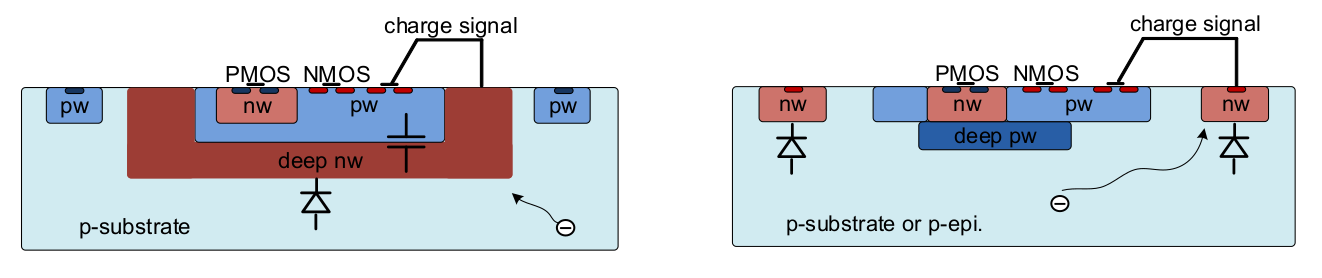
\includegraphics[width=15cm]{figures/Pixel_detectors/large_small_sensor_scheme.png}
         \caption{Concept cross-section of CMOS MAPS with large and small fill factor}
         \label{fig:large_small_sensor_scheme}
      \end{figure}
      To implement a uniform and stronger electric field, DMAPS often uses large electrode design that requires multiple wells (typically four including deep n and p wells); with this layout the total capacity of the sensor increases because of the addition of a new term (fig. \ref{fig:DMAPS_capacity}), which contributes to the total amplifier input capacity ($\sim$\SI{100}{fF}). In addition to the capacity between pixels ($C_{pp}$) and between the pixel and the backside ($C_{b}$), a non-negligible contribution comes from the capacities between wells ($C_{SW}$ and $C_{WW}$) needed to shield the embedded electronics. These capacities affect the thermal and 1/f noise of the charge amplifier and the $ \tau_{CSA}$ too:

      \begin{equation}
         ENC^2 _ {thermal} \propto \frac{4}{3}\frac{kT}{g_m}\frac{C_D ^2}{\tau_{sh}}
         \hspace{55pt}
         \tau_{CSA} \propto \frac{1}{g_m}\frac{C_D}{C_f}
      \end{equation}
      where $g_m$ is the transconductance, $\tau_{sh}$ is the shaping time. 
      Among the disadvantages coming from this large input capacity there is a coupling between the sensor and the electronics resulting in cross talk noise on neighbouring electrodes; indeed, since digital switching in the FE electronics does a lot of oscillations, this problem is especially connected with the intra wells capacities.
      \begin{figure}[h!]
         \centering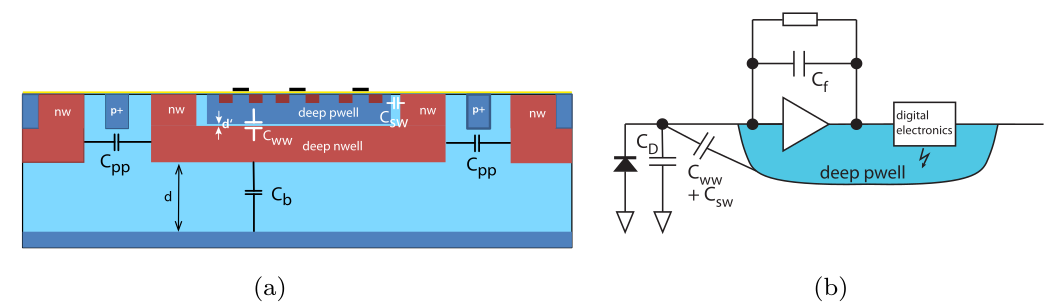
\includegraphics[width=12cm]{figures/Pixel_detectors/DMAPS_capacity.png}
         \caption{DMAPS scheme with shown the capacity terms ($C_{pp}$, $C_{b}$, $C_{WW}$, $C_{SW}$) which contribute to the total detctor capacity C$_{D}$}
         \label{fig:DMAPS_capacity}
      \end{figure}
      So, larger charge collection electrode sensors provide a uniform electric field in the bulk that results in short drift path and so in good collection properties, especially after irradiation, when trapping probability can become an issue.

      The small fill-factor variant, instead, benefits from a small capacity (\SIrange{5}{20}{fF}), but suffers from a non uniform electric field and from all the issue related to that (slowness and high trapping probability). 
      As we'll see these two different types of sensor require different amplifier: the large elcrtrode one is coupled with a charge sensitive amplifier, while the small one with a voltage amplifier (sec \ref{subsec:preamplifier}).

      \begin{table}
         \begin{center}
         \begin{tabular}{|c | c |c |}
         \hline
         & small fill factor & large fill factor\\
         \hline
         \hline
         small sensor C & $\surd$ ($<$ \SI{5}{fF}) & $\times$ ($\sim$ \SI{100}{200}{fF})\\
         low noise & $\surd$ & $\times$\\
         low cross talk & $\surd$ & $\times$ \\
         velocity perfomances & $\surd$ & $\times$ ($\sim$\SI{100}{ns})\\
         short drift paths & $\times$ & $\surd$ \\
         radiation hard & $\times$ & $\surd$ \\
         \hline
         \end{tabular}
         \caption{Small and large fill factor DMAPS characteristics}
         \label{tab:DMAPS_large_small_fillfactor}
         \end{center}
      \end{table}

   \subsection{A modified sensor}\label{chap:a_modified_sensor}
      A process modification, developed by CERN in collaboration with the foundries, which has become the standard solution to combine the characteristics of a small fill factor sensor (small input amplifier capacity) and of a large fill factor sensor (uniform electric field), is the one carried out for the ALICE upgrade for about ten years \cite{AProcessModification}.
      A compromise between the two sensors could also be making smaller pixels, but this solution requires reducing the electronic circuit area, so a completely new pixel layout should be though. The modification consists in inserting a low dose implant under the electrode and one of its advantage lies in its versatility: in fact, both standard and modified sensor are often produced for testing.

      Before the process modification, the depletion region extends below the diode towards the substrate, and it does not extend much laterally, even if a high bias is applied to the sensor (fig. \ref{fig:modified_process}). 
      After the modification, two distinct pn junctions are built: one between the deep p well and the n$^-$ layer, and the other between the n$^-$ and the p$^-$ epitaxial layer, extending to the whole area of the sensor.
      Since deep p well and the p-substrate are separated by the depletion region, the two p electrodes can be biased separately and this is beneficial to enhance the vertical electric field component.
      The doping concentration is an optimization parameter: it must be high enough to be larger than that in the epitaxial layer to prevent the punchthrough between p-well and the substrate, but it must also be low enough to allow the depletion for reasonable bias values.
      \begin{figure}
         \centering
         \begin{subfigure}[b]{0.52\textwidth}
             \centering
             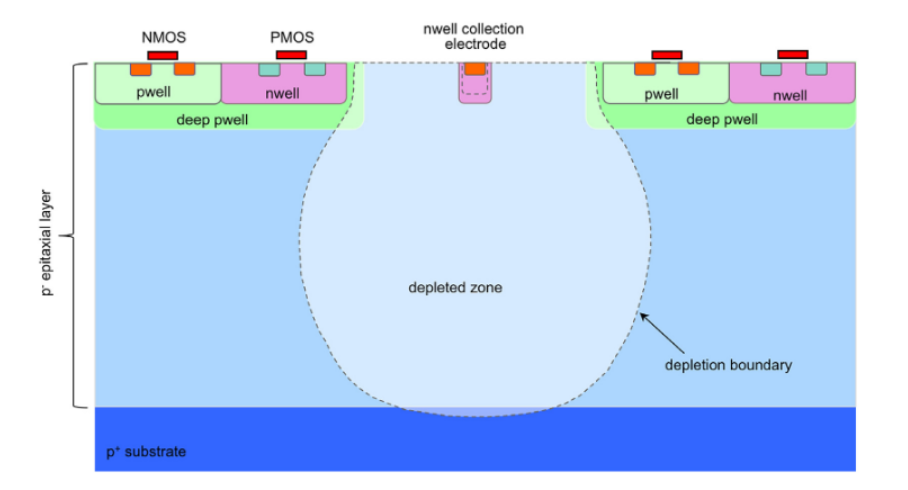
\includegraphics[width=\linewidth]{figures/Pixel_detectors/ALPIDE_before_PM.png}
             \caption{}
             \label{fig:ALPIDE_before_PM}
         \end{subfigure}
         \hfill
         \begin{subfigure}[b]{0.47\textwidth}
             \centering
             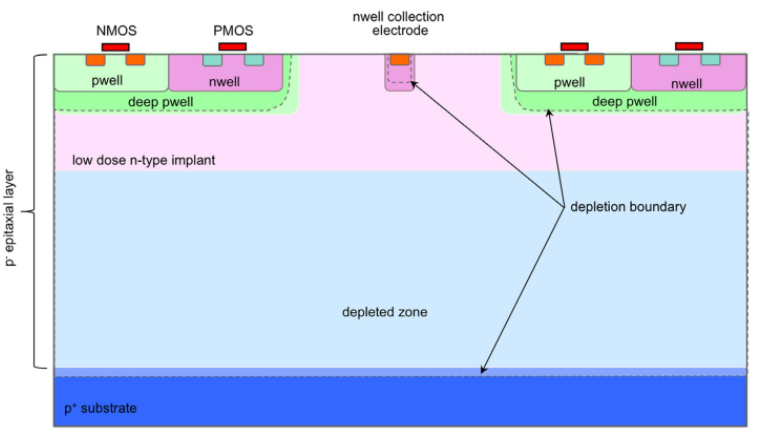
\includegraphics[width=\linewidth]{figures/Pixel_detectors/ALPIDE_after_PM.png} 
             \caption{}
             \label{fig:ALPIDE_after_PM}
         \end{subfigure}
         \label{fig:modified_process}
         \caption{A modified process for ALICE tracker detector: a low dose n implant is used to create a planar junction. In (a) it is difficult to deplete the epitaxial layer over its full
         width (b) the pixel is fully depleted.}
      \end{figure}

\section{Analog front end}
   After the collection on the electrode, the signal enters the front end amplification circuit (fig.\ref{fig:readout_scheme}), ready to be shaped and transmitted out of chip. Low noise amplification, fast hit discrimination and an efficient, high-speed readout architecture, consuming as low power as possible, are the goal of the readout integrated electronics (ROIC).
   \begin{figure}
      \centering
      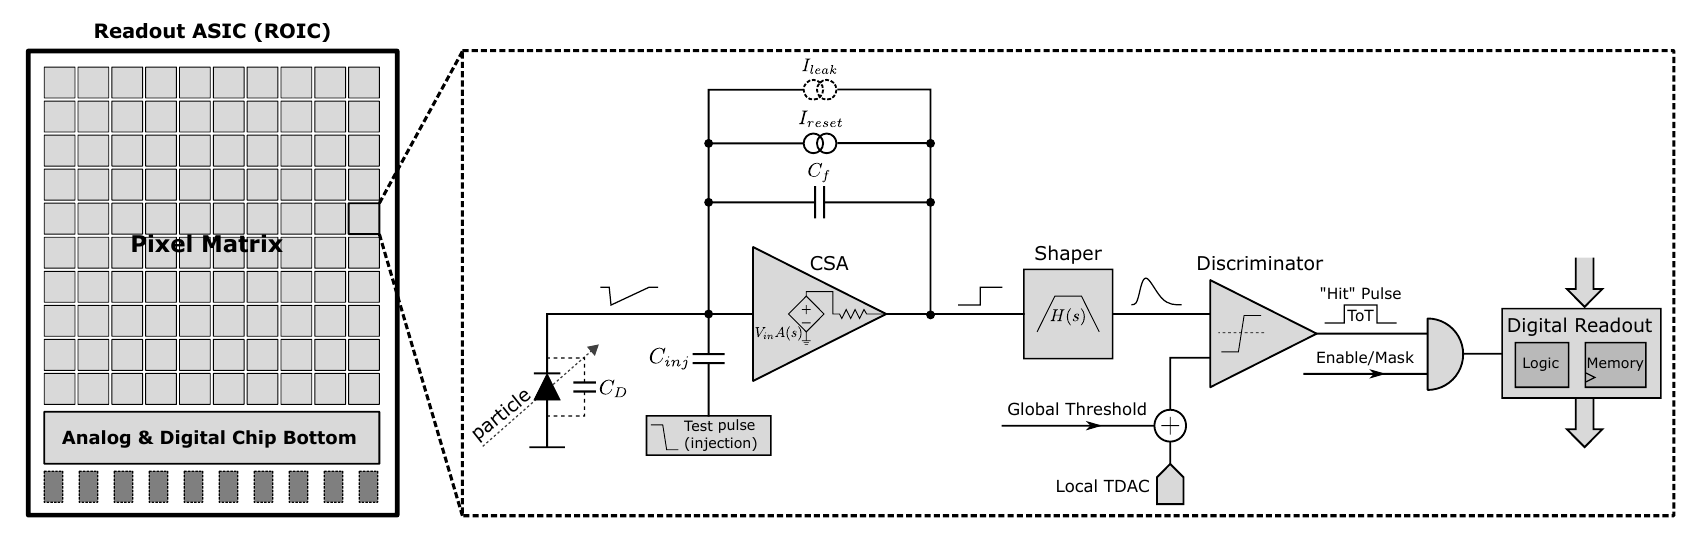
\includegraphics[width=1.\linewidth]{figures/Pixel_detectors/readout_scheme.png}
      \caption{Readout FE scheme: in this example the preamplifier is a charge sensitive one (CSA) but changing the capacitive feedback into a resistive one, this can be converted in a voltage or current amplifier.}
      \label{fig:readout_scheme}
   \end{figure}
   The main parts of the analog front end chain are a preamplifier (that often is the only amplification stage) with a reset to the baseline mechanism and a leakage current compensation, a shaper (a band-pass filter) and finally a discriminator. The whole chain must be optimized and tuned to improve the S/N ratio. It is very important both not to have a large noise before the amplification stage to avoid amplifying that noise, and to choose a reasonable threshold of the discriminator to cut noise-hits much as possible.

   \subsection{Preamplifier}\label{subsec:preamplifier}
      The a preamplifier can be designed as an operational amplifier (OpAmp) where the gain is determined by the input and feedback impedance (first step in figure \ref{fig:readout_scheme}):
      \begin{equation}
         G = \frac{v_{out}}{v_{in}} = \frac{Z_{f}}{Z_{in}}
      \end{equation}
      Depending on if a capacity or a resistance is used as feedback, respectively a charge or a voltage amplifier is used: if the voltage input signal is large enough and has a sharp rise time, the voltage sensitive preamplifier is preferred. Consequently, this flavor does not suit to large fill factor MAPS whose signal is small: $v_{in} = Q/C_{D} \approx$ \SI{3}{fC}/\SI{100}{pF} = \SI{0.03}{mV}, but it's fine for the small fill factor ones: $v_{in} = Q/C_{D} \approx$ \SI{3}{fC}/\SI{3}{pF} = \SI{1}{mV}.

      In the case of a resistor feedback, if the signal duration is longer than the discharge time ($\tau=R_S C_D$) of the detector the system works as current amplifier, as the signal is immediately trasmitted to the amplifier; in the complementary case (signal duration longer than the discharge time) the system integrates the current on the $C_D$ and operates as a voltage amplifier.
      
\section{Readout logic}
   The readout logic includes the part of the circuit which takes the FE output signal, processes it and then transmit it out of pixel and/or out of chip; depending on the situation of usage different readout characteristics must be provided. 
   To store the analogical information (i.e. charge collected, evolution of signal in time, ...) big buffers and a large bandwidth are needed; the problem that doesn't occur, or better occur only with really high rate, if one wants record only digital data (if one pixel is hit 1 is recorded, and if not 0 is recorded). 

   A common compromise is to store the time over threshold (ToT) of the pulse in clock cycle counts; this needs of relatively coarse requirement as the ToT can be trimmed down to use only a dozen bits but, being correlated with the deposited charge, it provides a sufficient information.
   The ToT digitalization usually takes advantage of the distribution of a clock (namely BCID,  bunch crossing identification) on the pixels' matrix. The required timing precision is better than $\sim$\SI{25}{ns}, that corresponds to the period between bunch collisions at LHC; for such reason a reasonable BCID-clock frequency for pixels detector is \SI{40}{MHz}.
   \begin{figure}[h!]
      \centering
      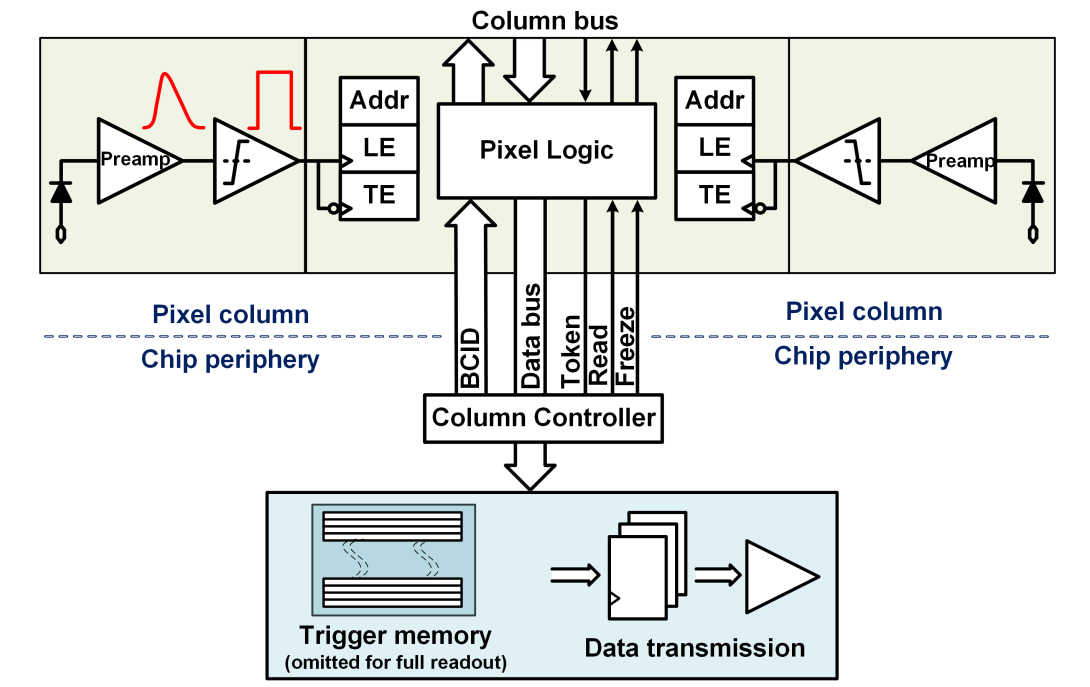
\includegraphics[width=.7\linewidth]{figures/Pixel_detectors/column_drain_RO.png}
      \caption{Column drain R/O scheme where ToT is saved}
      \label{fig:column_drain_RO-like}
   \end{figure}

   Moreover, the readout architecture can be full, if every hit is read, or triggered, if a trigger system decides if the hit must be stored or not. On one hand the triggered-readout needs buffers and storage memories,  hand the full readout, because there is no need to store hit data on chip, needs an high enough bandwidth.
   A triggered readout is fundamental in accelerator experiments where the quantity of data to store is very large and some selection has to be applied by the trigger: to give an order of magnitude, at LHC more than 100 TBit/s of data are produced, but the storage limit is about 100 MBit/s \cite{K-Wermes}\red{(pag. 797)}.
   Typically, the trigger signal is processed in a few $\mu s$, so the pixel gets it only after a hundred clock cycles from the hit arrival time: the buffer depht must be able to handle such high trigger latency. 
 
   After having taken out the data from the pixel, it has to be transmitted to the end of column (EoC) where a serializer delivers it out of chip, typically to an FPGA.
   There are several ways of transmitting data from a pixel to the EoC: a common one is the column-drain read out, developed for CMS and ATLAS experiments \cite{column-drain}. 
   All the pixels in a double-column share a data bus and only one pixel at a time, according to a priority chain, can be read. The reading order circuit is implemented by shift register (SR): when a hit arrives, the corresponding data, which can be made of timestamp and ToT, is temporarily stored on a RAM until the SR allows the access to memory by data bus. 
   Even if many readout architectures are based on the column-drain one, it does not work for large size matrices. The problem is the increasing number of pixels on a column would also raise the number of pixels in the priority chain, which would result in a slowdown of the readout. 

   If there isn't any storage memory, the double-column behaves as a single server queue and the probability for a pixel of waiting a time $T$ greater than $t$, with an input hit rate on the column $\mu$ and an output bandwidth $B_W$ is \cite{Garcia-Review}:
   \begin{equation}
   P(T > t) = \frac{\mu}{B_W} e^{-( B_W-\mu )t}
   \label{eq:priority_chain_no_buffer}
   \end{equation}
   To avoid hit loss (let's neglect the contribution to the inefficiency of the dead time $\tau$ due to the analog Front End), for example imposing $P_T > t\sim\:$0.001, one obtains $(B_W -\mu)\:t_t\sim\:$6, where $t_t$ is the time needed to transfer the hit; since $t_t$ is small, one must have $B_W \gg \mu$, that means a high bandwidth \cite{Garcia-Review}.
   \begin{figure}[h!]
      \centering
      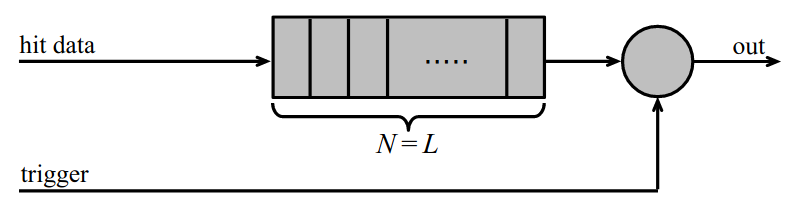
\includegraphics[width=.6\linewidth]{figures/Pixel_detectors/pipeline.png}
      \caption{Block diagram of a pipeline buffer: N is the dimension of memory buffer and L is the trigger latency expressed in BCID cycles}
      \label{fig:pipeline}
   \end{figure}

   Eq.\ref{eq:priority_chain_no_buffer} is actually an approximation, since each pixel sees a different bandwidth depending on the position on the queue: the first one sees the full bandwidth, while the next sees a smaller one because it can be occasionally blocked by the previous pixel. Then, the bandwidth seen by the pixel $i$ is $B_{i} = B - \sum _{j}\mu_{j}$, where $\mu_j$ is the hit rate of the $j$th pixel.
   The efficiency requirement on the bandwidth and the hit rate becomes: $B_{W,i} > \mu_{i}$, where the index $i$ means that the constraint is for a single pixel; if all the N pixels on a column have the same rate $\mu = N\mu_{i}$, the condition reduces to $B_{W} > \mu$.
   The bandwidth must be chosen such that the mean time between hits of the last pixel in the readout chain is bigger than that.
   In order to reduce the bandwidth, a readout with zero suppression on pixel is typically employed; this means that only information from channels where the signal exceeds the discriminator threshold are stored. 

   If, instead, the signal is locally stored until a trigger signal arrives, the input rate to column bus $\mu '$ is reduced compared to the hit rate $\mu$ as: $\mu'=\mu \times r \times t$, where $r$ is the trigger rate and $t$ is the bunch crossing period.
   In this situation there is a more relaxed constraint on the bandwidth, but the limiting factor is the buffer depth: the amount of memory designed depends both on the expected rate $\mu$ and on the trigger latency $t$ as $\propto\mu \times t$, which means that the higher the trigger latency the lower the hit rate to cope with. 

   In order to have an efficient usage of memory on pixels' area it's convenient grouping pixels into regions with shared storage. Let's compare two different situations: in the first one a buffer is located on each pixel area, while in the second one a core of four pixels share a common buffer (this architecture is commonly called FE-I4). \\
   \begin{figure}[h!]
      \centering
      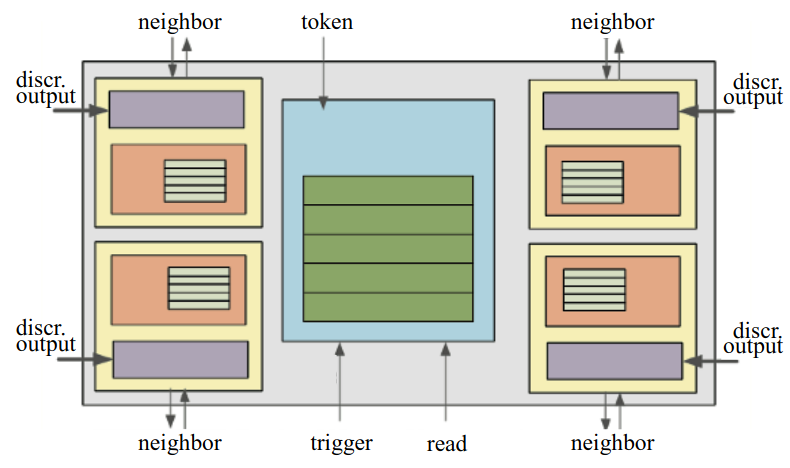
\includegraphics[width=.7\linewidth]{figures/Pixel_detectors/core.png}
      \caption{Block diagram of the FE-I4 R/O. Read and memory
      management section is highlighted in light blue; latency counters and
      trigger management secrion are highlighted in green; hit processing blocks
      are highlighted in purple; ToT counters and ToT management units are
      highlighted in orange}
      \label{fig:core}
   \end{figure}
   Consider a 50 kHz single pixel hits rate and a trigger latency of 5 $\mu s$, the probability of losing hits is: 
   \begin{equation}
      P(N > 1 | \nu) = 1-P(N = 0 | \nu) - P(N = 1 | \nu) = 1 - e^{-\nu} (1+\nu) \thickapprox 2.6 \% 
   \end{equation}    
   where I have assumed a Poissonian distribution with mean $\nu$ = 0.25 to describe the counts N.\\
   To get an efficiency $\epsilon$ greater than 99.9 \% a 3 hit depth buffer is needed: 
   \begin{equation}
      P(N > 3 | \nu) = 1-\sum_{i=0}^{3} P(N = i | \nu) < 0.1\%  
   \label{eq:efficiency_buffer}
   \end{equation} 
   Consider the second situation: if the average single pixel rate is still \SI{50}{kHz}, grouping four pixels the mean number of hits per trigger latency is $\nu = 0.25 \times 4 = 1$. To get an efficiency of 99.9\% (eq. \ref{eq:efficiency_buffer}) a buffer depth of 5 hits in the four-pixels region, instead of 3 per pixels, is needed. 

